\documentclass[11pt]{article}
\usepackage[utf8]{inputenc}
\usepackage{parskip}
\usepackage[a4paper, margin=1in]{geometry}
\usepackage{graphicx}
\usepackage{hyperref}
\usepackage{listings}
\usepackage{array}
\usepackage[capitalise,noabbrev]{cleveref}
\usepackage{rotating}

% Custom json syntax highlightning
\usepackage{bera}
\usepackage{xcolor}

\colorlet{punct}{red!60!black}
\definecolor{background}{HTML}{EEEEEE}
\definecolor{delim}{RGB}{20,105,176}
\definecolor{string}{RGB}{61,107,42}
\colorlet{numb}{magenta!60!black}

\lstdefinelanguage{json}{
    basicstyle=\normalfont\ttfamily,
    % numbers=left,
    % numberstyle=\scriptsize,
    % stepnumber=1,
    % numbersep=8pt,
    showstringspaces=false,
    breaklines=true,
    frame=lines,
	backgroundcolor=\color{background},
	string = [d]{"},
	stringstyle={\color{string}},
    literate=
     *{0}{{{\color{numb}0}}}{1}
      {1}{{{\color{numb}1}}}{1}
      {2}{{{\color{numb}2}}}{1}
      {3}{{{\color{numb}3}}}{1}
      {4}{{{\color{numb}4}}}{1}
      {5}{{{\color{numb}5}}}{1}
      {6}{{{\color{numb}6}}}{1}
      {7}{{{\color{numb}7}}}{1}
      {8}{{{\color{numb}8}}}{1}
      {9}{{{\color{numb}9}}}{1}
      {:}{{{\color{punct}{:}}}}{1}
      {,}{{{\color{punct}{,}}}}{1}
      {\{}{{{\color{delim}{\{}}}}{1}
      {\}}{{{\color{delim}{\}}}}}{1}
      {[}{{{\color{delim}{[}}}}{1}
      {]}{{{\color{delim}{]}}}}{1},
}


\renewcommand{\arraystretch}{1.5}

\title{Task 2 Report}
\date{\today}
\author{Federico Fregosi, Mirko Laruina,\\
        Riccardo Mancini, Gianmarco Petrelli}

\begin{document}
\pagenumbering{gobble}
\maketitle
\vfill
% \setcounter{tocdepth}{1}
\tableofcontents
\vfill
\clearpage
\setcounter{page}{1}
\pagenumbering{arabic}

\section{Specifications}

\subsection{Application Overview}
The application is an aggregator of movies and movie ratings with the purpose 
of providing logged users statistics and informations about a large set of movies.
Logged-in user can also rate movies they have watched while not logged-in users 
may still use the service to browse movie rankings and statistics but they are not
able to give their rate. Only movies released in Italy are considered.

All users can search a movie and view its details (e.g., title, original title, duration, 
cast, ...) along with its aggregated statistics about ratings. 

In addition, all users can browse the list of movies sorting and filtering it by many parameters
(e.g. year, genre, country, actors, ...).

System administrators can view all user pages and ban users. In order to do that, he can 
check the full history of ratings.

The movie database will be built upon the publicly available IMDb dataset.

The ratings will be gathered also by periodically scraping other websites 
(e.g., Rotten Tomatoes, Coming Soon, MyMovies).

\subsection{Actors}
Anonymous user, registered user, administrator and bot.

\subsection{Requirement Analysis}

\subsubsection{Functional Requirements}
An \textbf{anonymous user} must be able to register in order to become a 
\textit{registered user}. Login is carried out using username and password selected 
by the user when registering. Username must be unique. A valid email address is
also required in order to register. An email cannot be used more than once.

Both \textbf{anonymous user} and \textbf{registered user} must be able to:
\begin{itemize}
	\item view details and average rating of a specific movie
	\item view a list of movies and filter it by many parameters. Combined filters 
	are also allowed
	\item view aggregated statistics about movies grouped by year, country, actor,
	director, genre 
\end{itemize}

A \textbf{registered user} must be able to rate a movie, in addition to what anonymous
user can do. A registered user must also be able to manage his profile. In the profile a
registered user can:
\begin{itemize}
	\item check, add and modify his personal data
	\item browse the history of his rates
	\item view aggregated statistics about his profile (i.e. most viewed genre,
	most recurrent actor, etc...) based on his rated movies
	\item delete the account
\end{itemize}
Finally, a registered user can logout in any moment.

An \textbf{administrator} is a special registered user who must be able to ban users.
In order to do that, an administrator can check a global rating history to retrieve information
about all the application's activity, and to check every user's profile.
Banned user's rating are automatically removed from the database. Email and username
of banned users cannot be used again.

The \textbf{bot} is not a real user but an entity used to periodically update the database in order to add new movies and update external ratings. 

\subsubsection{Non-Functional Requirements}
\begin{itemize}
	\item Availability: the Database must be replicated in order to be always available.
	Write operations on the Database can be eventually consistent.
	\item Scalability: the application must be able to scale to an arbitrary number of servers.
	\item Security: passwards must be stored in a secure way.
	\item Responsive UI: Client-side application must provide a responsive view both for pc, 
	laptops and mobile devices.
\end{itemize}

\section{Design}

\subsection{Use-case diagram}

\begin{sidewaysfigure}[h!]
    \centering
    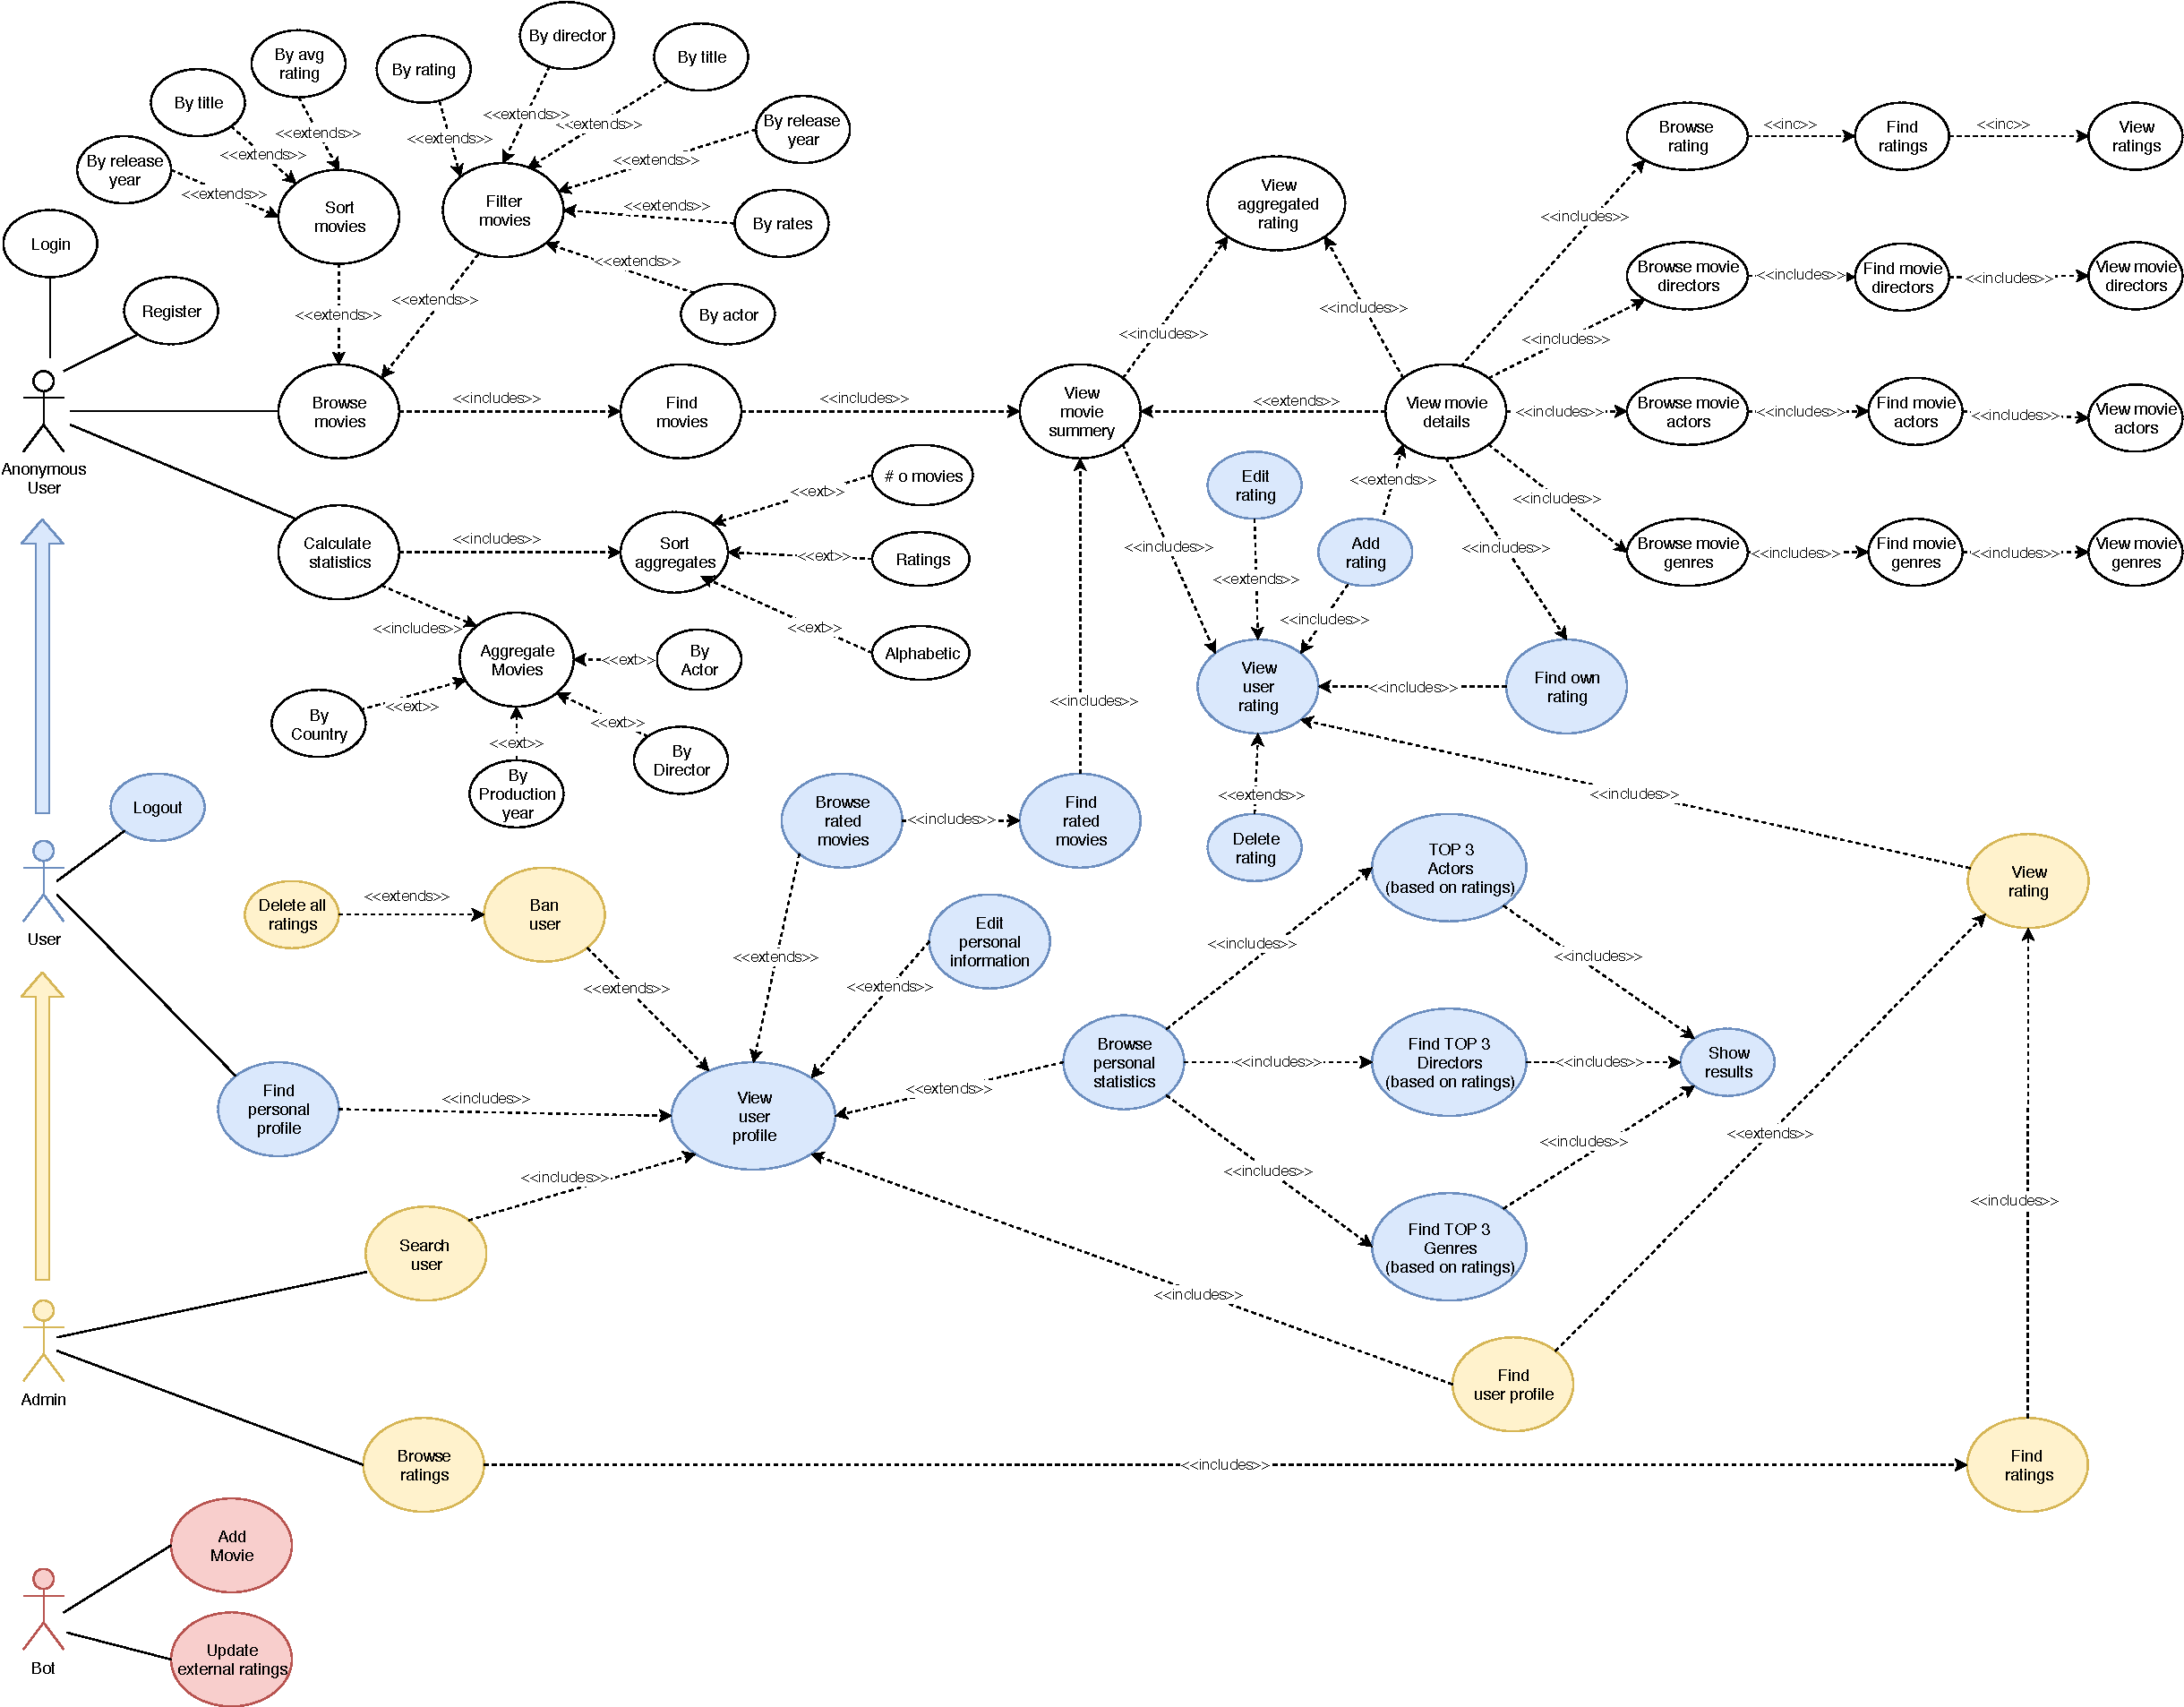
\includegraphics[height=18cm]{figs/use_case.pdf}
    \caption{Use-case diagram}
    \label{fig:usecase}
\end{sidewaysfigure}

The use-case diagram is shown in \cref{fig:usecase}. Different colors are used to highlight cases that are exclusive of some actors: blank cases are referred to all users; blue cases are referred to registered user and admin; yellow cases are exclusive of the admin.

\subsection{Class diagram}

\begin{figure}[h!]
    \centering
    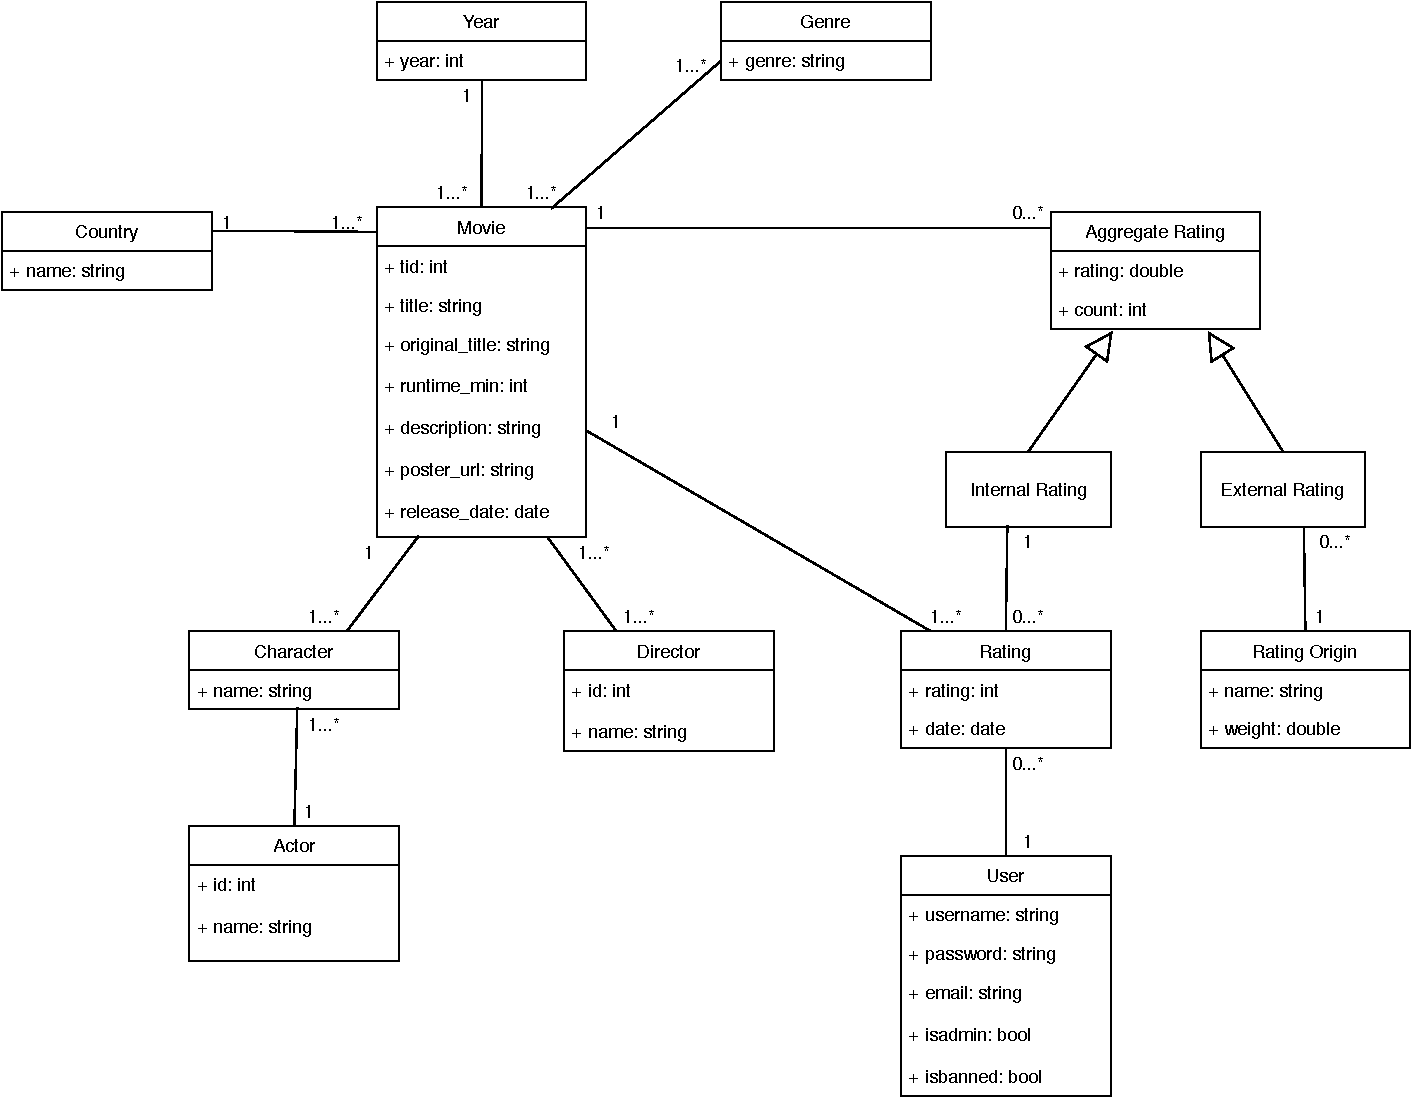
\includegraphics[width=\textwidth]{figs/class_diagram.pdf}
    \caption{Class diagram for the identified entities}
    \label{fig:class_diagram}
\end{figure}

The class diagram is shown in \cref{fig:class_diagram}. It was decided to show \emph{Country}, \emph{Year} and \emph{Genre} as separate entities as they are some of the fields over which aggregate statistics are calculated. In the database implementation, this will reflect in having a separate collection for each of them in which pre-computed results of the aggregations will be stored.

\clearpage
\subsection{Data model}
The data model is split in 9 different collections:
\begin{itemize}
	\item Movies (\cref{sec:movies})
	\item Users (\cref{sec:users})
	\item Ratings (\cref{sec:ratings})
	\item Actors (\cref{sec:actors})
	\item Directors (\cref{sec:directors})
	\item Years (\cref{sec:years})
	\item Genres (\cref{sec:genres})
	\item Countries (\cref{sec:countries})
	\item BannedUsers (\cref{sec:banned_users})
\end{itemize}
In each following subsection, an example document is shown for every collection.

\subsubsection{Movies}
\label{sec:movies}

\begin{lstlisting}[language=json]	
{
	_id: 7286456,
	title: "Joker",
	original_title: "Joker",
	runtime: 122,
	region: "US",
	full_region: "USA",
	year: 2019,
	date: "2019-10-04",
	description: "In Gotham City, mentally troubled comedian [...]",
	poster: "https://m.media-amazon.com/images/M/[...].jpg",
	characters: [
		{
			name: "Joker",
			actor_name: "Joaquin Phoenix",
			actor_id: 1618
		},
		...
	],
	directors: [
		{
			id: 680846,
			name: "Todd Phillips",
		}
	],
	genres: ["Crime", "Drama", "Thriller"],
	ratings: [
		{
			source: "internal",
			avgrating: 9,
			count: 100,
			weight: 2
		},
		{
			source: "IMDb",
			avgrating: 8.6,
			count: 628981,
			weight: 1
		},
		...
	],
	total_rating: 8.87
}
\end{lstlisting}

\paragraph{Notes}
Character and director nested documents contain redoundant data (person's name) that is introduced to reduce the number of seeks necessary to return the movie details
to the user.

This collection is mainly read-heavy since most fields will be written only once.
The only fields subject to change are the ones related to ratings. For these reasons,
we can affort many indices to speed-up the aggregations.

\paragraph{Indices} 
Indices on the following fields will be set for this collection:
\begin{itemize}
	\item \texttt{title}
	\item \texttt{region}
	\item \texttt{year}
	\item \texttt{characters.actor\_id} (multikey index)
	\item \texttt{directors.id} (multikey index)
	\item \texttt{total\_rating}
\end{itemize}

An index on the \emph{total rating} is necessary for efficiently returning a 
subset of movies based on their rating. However, frequent writes on it would 
negatively impact the performance on the system. Therefore, this field will 
not contain the real-time total rating but will be updated periodically.

\subsubsection{Users}
\label{sec:users}

\begin{lstlisting}[language=json]	
{
	_id: <ObjectId>,
	username: "joker",
	password: "<HASHED PASSWORD>",
	email: "joker@dccomics.com",
	isadmin: 1 (optional)
}
\end{lstlisting}
% top_actors: [
% 	{
% 		name: "Joaquin Phoenix",
% 		id: 1618
% 	},
% 	...
% ],
% top_directors: [
% 	{
% 		id: 680846,
% 		name: "Todd Phillips",
% 	},
% 	...
% ],
% top_genres: ["Crime", "Drama", "Thriller"]
% }

% TODO controlla che abbia senso

\paragraph{Indices} 
An index will be introduced on the \emph{username} and \emph{email} fields. 
Furthermore, these fields must also be unique.

\subsubsection{Ratings}
\label{sec:ratings}

\begin{lstlisting}[language=json]	
{
	_id: <ObjectId>,
	user_id: <ObjectId>,
	movie_id: 7286456,
	date: "2020-01-20",
	rating: 10
}
\end{lstlisting}

\paragraph{Notes}
The raw ratings are kept separated from the movie they refer to because the single 
ratings are never shown to the user. 
Furthermore, new ratings are expected to be frequently added.
By using a separate collection, the problem of a long array of nested documents 
is avoided. However, the introduction of an index is necessary.


\paragraph{Indices} 
An index will be introduced on the \emph{movie\_id} field in order to speed up
aggregations.

\subsubsection{Actors}
\label{sec:actors}

\begin{lstlisting}[language=json]	
{
	_id: 1618,
	name: "Joaquin Phoenix",
	avg_rating: 8.75,
	movie_count: 17
}
\end{lstlisting}

\paragraph{Notes}
This collection will store the pre-computed results of the aggregation.

\subsubsection{Directors}
\label{sec:directors}

\begin{lstlisting}[language=json]	
{
	_id: 680846,
	name: "Todd Phillips",
	avg_rating: 7.45,
	movie_count: 4	
}
\end{lstlisting}

\paragraph{Notes}
This collection will store the pre-computed results of the aggregation.

\subsubsection{Years}
\label{sec:years}

\begin{lstlisting}[language=json]	
{
	_id: 2019,
	avg_rating: 6.45,
	movie_count: 867
}
\end{lstlisting}

\paragraph{Notes}
This collection will store the pre-computed results of the aggregation.

\subsubsection{Genres}
\label{sec:genres}

\begin{lstlisting}[language=json]	
{
	_id: "Crime",
	avg_rating: 4.78,
	movie_count: 751
}
\end{lstlisting}

\paragraph{Notes}
This collection will store the pre-computed results of the aggregation.

\subsubsection{Countries}
\label{sec:countries}

\begin{lstlisting}[language=json]	
{
	_id: "US",
	full_name: "USA",
	avg_rating: 4.78,
	movie_count: 1597
}
\end{lstlisting}

\paragraph{Notes}
This collection will store the pre-computed results of the aggregation.

\subsubsection{BannedUsers}
\label{sec:banned_users}

\begin{lstlisting}[language=json]	
{
	_id: <ObjectId>,
	username: "topolino.hackerino",
	email: "hackerino@topolino.it"
}
\end{lstlisting}

\paragraph{Notes}
This collection stores the username and passwords of banned users. 
When a user is banned, its record in the \emph{Users} collection is moved
to this one.
When a new user registers, this collection is checked for any match and, 
if any is found, the registration will fail. 

\subsection{Software Architecture}

%DUBBI
%username must be unique? (functional or not functional?)
%->unique, functional, inserire anche in task 1
%the only difference between anonymous and registered user is that reg. user can rate?
%->+profile with stats on him
%can a film be marked as watched?
%->no
%email is necessary for registration?
%->yes + personal informations (not required)

\end{document}